\documentclass{article}
\usepackage[margin=1in]{geometry}
\usepackage{fancyhdr}
\usepackage{graphicx}
\usepackage{vhistory}
\usepackage[parfill]{parskip}
\graphicspath{{./}}

% Set fancy looking header/footer and move page number to the right
\pagestyle{fancy}
\fancyhead{}
\fancyfoot{}
\fancyfoot[R]{\thepage}

\title{}
\author{}
\date{}

\begin{document}

    % For large document with titlepage:
    \pagenumbering{gobble}
    \begin{titlepage}
    \begin{center}
        \vspace*{1cm}

        \Huge
        \textbf{User's Guide for Cloud Backup}

        \vspace{.5cm}
        \LARGE
        Captain CyBeard: Neil Before Us

        \vspace{1cm}

        \textbf{Ryan Breitenfeldt \textbar\ Noah Farris\\ Trevor Surface \textbar\ Kyle Thomas}

        \vspace{.2cm}
        \Large
        May 4, 2020

        \vspace{2cm}
        
\includegraphics[scale=1]{logo}

        \vfill

        Washington State University Tri-Cities\\
        CptS 423 Software Design Project 2

    \end{center}
\end{titlepage}



    \tableofcontents
    \listoffigures

    \newpage
    \begin{versionhistory}
        \vhEntry{0.3}{10.15.2019}{TS}{Completed Overview}
        \vhEntry{0.2}{10.10.2019}{RB NF TS KT}{Filled in Environment \& Operation sections}
        \vhEntry{0.1}{09.27.2019}{KT}{Document Creation}
    \end{versionhistory}
    \newpage

    \pagenumbering{arabic}
    \section{Introduction}
    The requirements specification document is to go over the requirements for %%%%%%%%%%%%%%%%%%%%%%%%%%%%%%%%%%%%
    This application is to give the user the ability to download their virtual machines for upload to Cypherpath’s resiliency platform.
    It will be a Django web application in Python3. The user will be able to get the virtual machines they have in the VMware cloud and AWS cloud.
    It should detect what service is from the URL supplied by the user. The user will be given a selectable list of virtual machines on
    their desired cloud service for them to chose from. The user will select from the list and download the wanted virtual machine.
    The virtual machine will then be downloaded to the local computer. The requirements from Cypherpath are detailed here in how Cypherpath desires to
    accomplish this program. This program will later be expanded by Cypherpath to be integrated into their software.     
    

    \section{Background}
	This project aims to give Cypherpath users a simple means of retrieving Virtual Machine snapshots from different websites while making it easy to 
	then upload those snapshots to Cypherpath's software, providing more value to the customer in the process.


    \section{Overview}
    The purpose of this application is to allow users to download files from online Virtual Machines (VM), to local file storage.
    The application itself will operate in the web browser using Python3 and Django. Upon starting the application the user would
    provide a URL of their VM. Processing the URL the user is then asked to provide credentials to validate they are the owner of
    the VM. After completing the verification, the application will then use the API of the client the user has their VM stored on
    to access their folders. The User will be shown their folder structure and chose to download the files locally to their desktop.
    Upon accepting to download locally the application will use another API to download the files local to their VM.

    The application will be written with Django and Python3, including the requests libraries for API calls, SAML for Authentication
    and standard libraries.

    The application only allows users to view the files from VM's they own, and download those file locally to the machine they 
    are running the application through. The users will have the ability to provide either a VMWare URL to download from, or an
    Amazon Web Services (AWS) VM URL. The application will be designed with modularity in mind to allow further 
    development with different VM service providers.  


    \section{Environment}
    The environment that the software will preside in consists of modules to interact with \textbf{VMWare}, 
    \textbf{AWS}, other virtual machine platforms and will also be interacting with authentication modules for those
    various platforms. The user will interact with the API's of these cloud services and authentication
    methods through a Django Web App. Lastly, the environment will consist of the application storing the selected
    virtual machines onto the user's local machine.

    %%%%%%%%%%%%%%% DIAGRAM STILL NEEDS TO BE FIXED!!! %%%%%%%%%%%%%%%%%%%%%%%%%%
    \begin{figure}[h]
    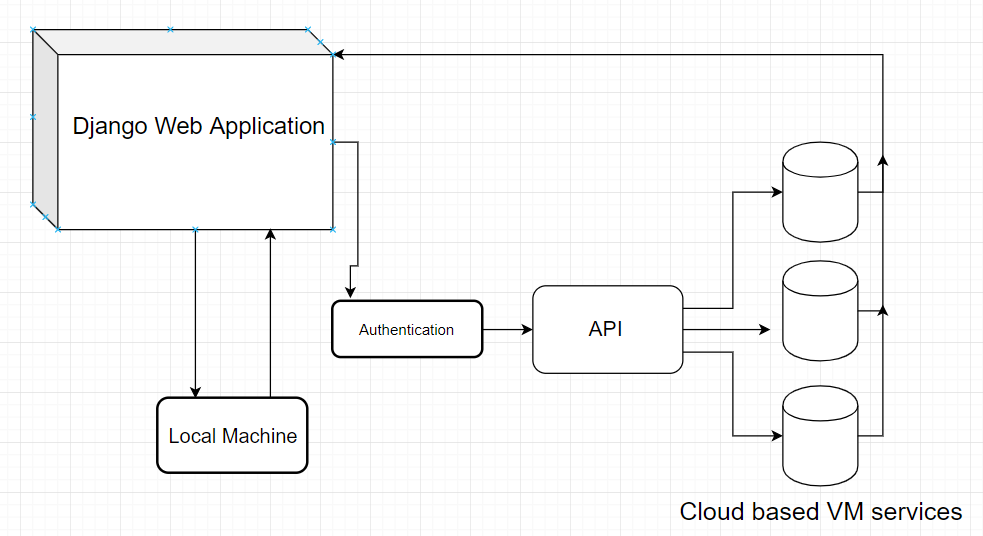
\includegraphics[scale=.7]{diagram}
        \caption{The application environment}
    \end{figure}
    %%%%%%%%%%%%%%% DIAGRAM STILL NEEDS TO BE FIXED!!! %%%%%%%%%%%%%%%%%%%%%%%%%%

        \subsection{VMWare (VSphere)}

            \subsubsection{API'S}
            Use VMWare API that looks at file structs.

%            Example URL:

            \subsubsection{Download Protocol}
            Call downloads to download to local machine.

        \subsection{AWS}
            \subsubsection{API'S}
            Use AWS API that looks at file structs.

            \subsubsection{Download Protocol}
            Call download API to download to local machine.

        \subsection{Authentication}
        The Application should retain a user's login token for the various platforms to minimize the frequency they need to authenticate to the different VM platforms.
        An option for them to log out of these sessions should also be provided.

            \subsubsection{VMWare Auth (SAML)}
            Use specific authorization based on the VMWare standard.

            \subsubsection{AWS Authentication}
            Use specific authorization based on the AWS standard.

        \subsection{Web Page}
            \subsubsection{Django}
            Provide input box for URL: should also provide login and logout usage.

        \subsection{Download Structure}

        \subsection{Database?}


    \section{Operation}
    In the following sections the operation of the application will be described, including starting the application
    (invocation), the commands the application uses and finally, how to close or terminate the application.

        \subsection{Invocation}
            \subsubsection{Web Application}

        \subsection{Commands}
            \subsubsection{Download}
            
            \subsubsection{Load File Structure}

            \subsubsection{Error Catching}

            \subsubsection{Authentication}

        \subsection{Termination}
            \subsubsection{Logout User}

            \subsubsection{Closing Application}

    \section*{References}
    % Reference the project plan?
    % Possibly reference documentation to the various API's?

    \appendix
    \section{Appendix}
    % Sample files, if any?
    % Maybe a sketch of the general page layout?

\end{document}
